\chapter{Experimental Setup}
\label{chap:setting}


For the proposed measurements, we require a large kinematic coverage for the 
scattered electrons and the ability to tag low momentum spectators. The CLAS12 
detector with 11~GeV electron beam is well suitable to access the valence 
region. A low energy recoil detector with good performance is the key parameter 
for the success of such measurements.

\section{CLAS12 Forward Detector}

The CLAS12 detector is designed to operate with 11~GeV beam at a 
electron-nucleon luminosity of $L = 1\times10^{35}$cm$^{-2}$s$^{-1}$. The 
baseline configuration of the CLAS12 detector consists of the Forward Detector 
and the Central Detector packages~\cite{CD} (see Fig.~\ref{fig:fd}).

\begin{figure}
  \begin{center}
    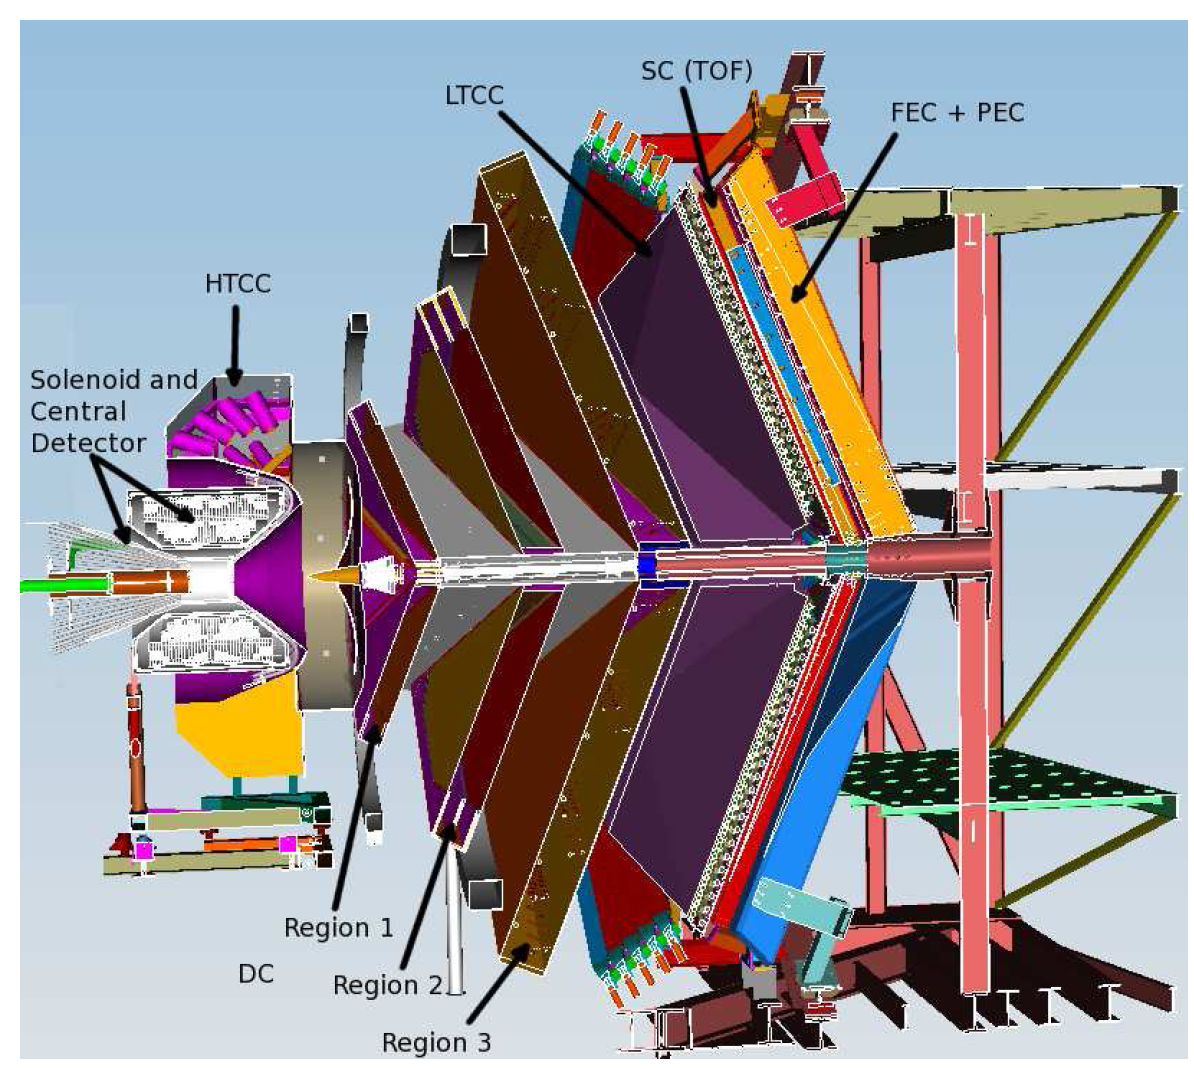
\includegraphics[angle=0, width=0.75\textwidth]{./../Detector/fig-chap2/fd}
    \caption{The schematic layout of the CLAS12 baseline design.}
    \label{fig:fd}
  \end{center}
\end{figure}

The scattered electrons will be detected in the forward detector which consists 
of the High Threshold Cherenkov Counters (HTCC), Drift Chambers (DC), the Low 
Threshold Cherenkov Counters (LTCC), the Time-of-Flight scintillators (TOF), 
the Forward Calorimeter and the Preshower Calorimeter. The charged particle 
identification in the forward detector is achieved by utilizing the combination 
of the HTCC, LTCC and TOF arrays with the tracking information from the Drift 
Chambers. The HTCC together with the Forward Calorimeter and the Preshower 
Calorimeter will provide pion rejection factor of more than 2000 up to momentum 
of 4.9 GeV, and a rejection factor of 100 above 4.9 GeV.

\section{Low Energy Recoil Detector}


In addition to the Forward Detector package, we require a low energy recoil 
detector which has adequate momentum and spatial resolution, and good particle 
identification for recoiling charged particles (p, $^2$H, $^3$H and $^3$He). We 
investigate the feasibility of using the CLAS12 Central Detector and the BoNuS 
Detector~\cite{bonus6,bonus12}. As those seem not suitable for the proposed 
measurement we propose a new detector for our measurement.

\subsection{Central Detector}


CLAS12 Central Detector~\cite{CD} is designed to detect various charged 
particles over a wide momentum and angular range. The main detector package 
includes:
\begin{itemize}
 \item Solenoid Magnet: provides a central longitudinal magnetic field up to 5 
    Tesla, serves to curl emitted low energy M{\o}ller electrons and determine 
    particle momenta through tracking.
 \item Central Tracker: consists of 3 layers of silicon strips and 3 layers of 
    Micromegas. The thickness of a single silicon layer is 
    $300\mu$m~\cite{SVT}.
 \item Central Time-of-Flight: an array of scintillator paddles with a 
    cylindrical geometry of radius 26 cm and length 50 cm, and the thickness of 
    the detector is 2 cm with designed timing resolution of $\sigma_t = 50$ ps, 
    used to separate pions and protons up to 1.2 GeV/$c$.
 \item Central Neutron Detector:  three radial layers of 3 cm thick 
    scintillator bars arranged cylindrically to identify neutrons above 200 
    MeV/c up to 1.2 GeV/c with 10\% momentum resolution.
\end{itemize}


However, the current design is not optimal for low energy particles ($p<300$ 
MeV/$c$) due to the energy loss in the first 2 silicon strips. The momentum 
detection threshold is $\sim 200$ MeV for protons, $\sim 350$ MeV for deuterons 
and even higher for $^3$H and $^3$He. These values are significantly too large 
for our proposed measurement, therefore other options should be explored.

\subsection{BoNuS 12 Radial Time Projection Chamber}

The original BoNuS detector was built for Hall B experiment E03-012 to study 
the neutron structure by scattering electrons off an almost on-shell neutron in 
the deuterium target. The purpose of the detector was to tag the resulting low 
energy protons ($p>60$ MeV/$c$). The key component for detecting the slow 
protons was the Radial Time-projection Chamber (RTPC) based on Gas Electron 
Multipliers (GEM). The second run period (EG6) used a $^4$He gas target and an 
improved RTPC to detect recoiling $\alpha$ particles in coherent scattering.  
The major improvements of the EG6 RTPC were full cylindrical coverage and 
higher data taking rate.

The approved 12~GeV BoNuS (BoNuS12) proposal is planning to use a similar 
device with some upgrades. The target gas cell length will be doubled, and the 
new RTPC will be longer as well, leading to a doubling in luminosity and an 
increased acceptance. Taking advantage of the larger bore ($\sim 700$ mm) of 
the CLAS12 5-Tesla solenoid magnet, the maximum radial drift length will be 
increased from the present 3 cm to 6 cm, improving the momentum resolution by 
50\%~\cite{bonus12} and extending the momentum coverage. The main features of 
the proposed BoNuS12 detector are summarized in Table~\ref{tab:bonus}.

\begin{table}
\center
\caption{\label{tab:bonus}Main features of the BoNuS 12 detector.}
\vspace*{0.2cm}
\begin{tabular}{|c|c|}
\hline
Radial drift length & 8 cm\\
\hline
longitudinal length & $\sim$ 40 cm\\
\hline
Gas mixture & 80\% helium/20\% DME\\
\hline
Azimuthal coverage & 2$\pi$\\
\hline
Momentum range & 70-250 MeV/$c$\\
\hline
DAQ rate & $\sim 3$kHz\\
\hline
Solenoidal field & $\sim 5$ T\\
\hline
Gas target length/diameter & $\sim$40 cm/6 mm\\
\hline
Target wall & 25 $\mu$m Kapton\\
\hline
Target window & 15 $\mu$m Al\\
\hline
Target pressure & 7.5 atm\\
\hline
\end{tabular}
\end{table}


The results from the 2005 BoNuS and 2009 EG6 run demonstrate the successful 
performance of the RTPC. The agreement between the vertex trajectory for a 
recoiling $^4$He and the electron in CLAS is shown in 
Fig.~\ref{fig:EG6elastic_delta} from EG6.  

\begin{figure}
  \begin{center}
    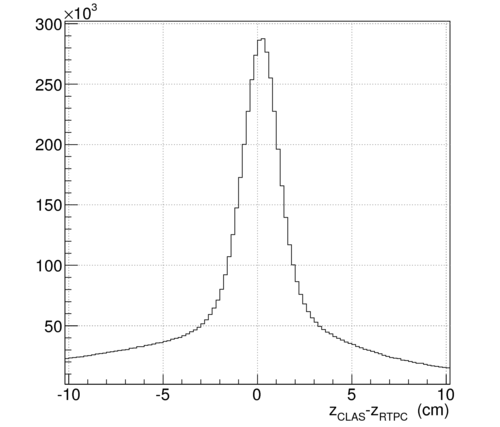
\includegraphics[angle=0, width=0.32\textwidth]{./../Detector/fig-chap2/eg6elastic_dz_small}
    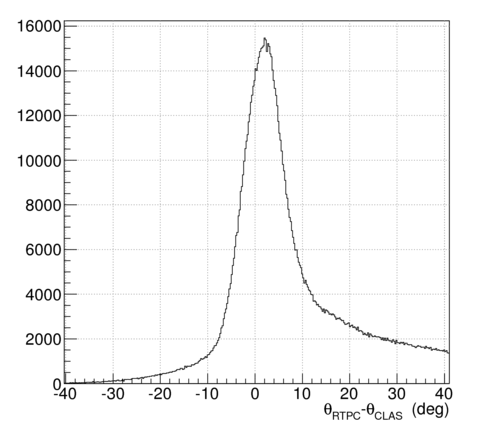
\includegraphics[angle=0, width=0.32\textwidth]{./../Detector/fig-chap2/eg6elastic_dthe_small}
    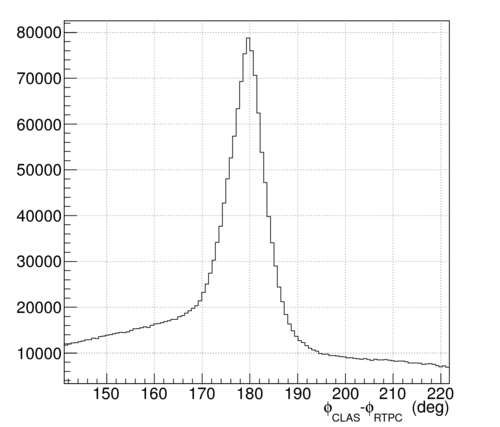
\includegraphics[angle=0, width=0.32\textwidth]{./../Detector/fig-chap2/eg6elastic_dphi_small}
    \caption{Difference between the reconstructed vertex trajectory ($z$,$\theta$,$\phi$) measured by EG6's RTPC and that calculated from CLAS's electron for $^4$He data at 1.2 GeV.\label{fig:EG6elastic_delta}}
  \end{center}
\end{figure}


In principle, particle identification can be obtained from the RTPC through the 
energy loss $dE/dx$ in the detector as a function of the particle momentum (see 
Fig.~\ref{fig:eloss}). However, this necessitates gain calibration, which 
according to the BoNuS study, varies a lot over the surface of the detector.  
This is likely due to the GEM gain variations across different regions arising 
from slight misalignments and wrinkles. The upgraded EG6 detector also exhibits 
this characteristic, shown in Fig.~\ref{fig:EG6gains}. Yet, even with perfect 
calibration, because we actually measure the curvature $\propto p/Z$ and not 
the momentum, $^3$H and $^3$He curves are very close (see 
Fig.~\ref{fig:eloss}). Such a small difference is impossible to discriminate on 
an event by event basis because of the intrinsic width of the $dE/dx$ 
distributions. This feature is not problematic when using the deuterium target, 
but makes the RTPC improper for our measurement on the helium 4 target.


Another issue with the RTPC is its slow response time due to the drift time 
($\sim 5\mu$s). Indeed, a much faster recoil detector could be included in the 
trigger and have significant impact on background rejection. Since data 
acquisition speed was the main limiting factor for both BoNuS and EG6 runs in 
CLAS, including the recoil detector in the trigger would allow to run at higher 
luminosities. Indeed events without a hit in the recoil detector would not be 
recorded and reduce the trigger frequency significantly.

\begin{figure}
  \begin{center}
    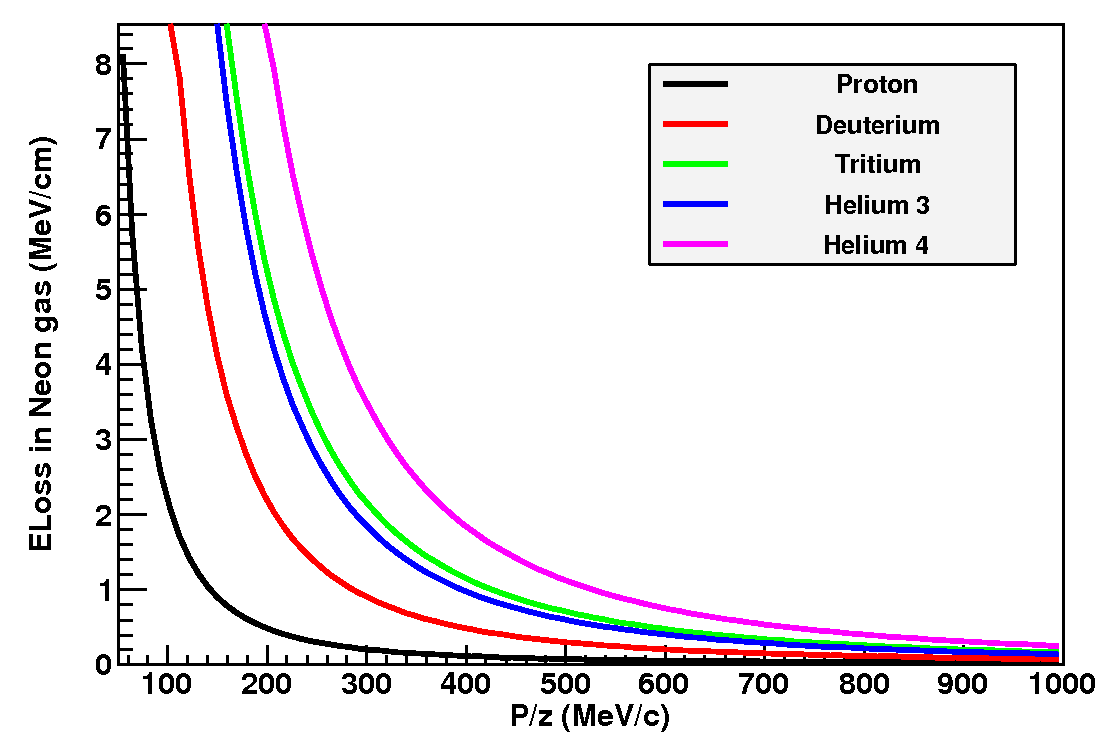
\includegraphics[angle=0, width=0.5\textwidth]{./../Detector/fig-chap2/pz}
    \caption{Calculation of energy loss in Neon gas as a function of the particle momentum divided by its charge for different nuclei. }
    \label{fig:eloss}
  \end{center}
\end{figure}

\begin{figure}
  \begin{center}
    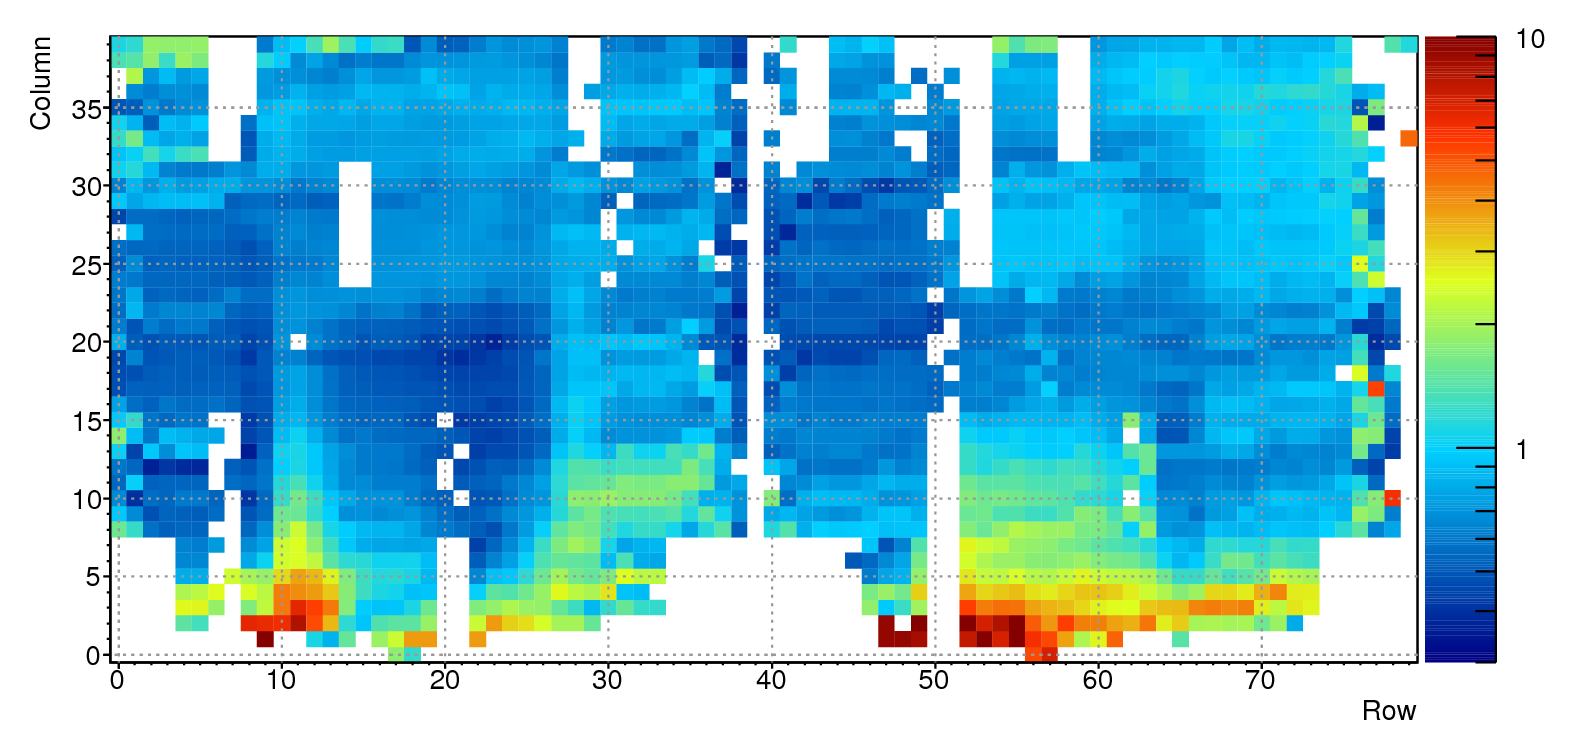
\includegraphics[angle=0, width=0.8\textwidth]{./../Detector/fig-chap2/eg6_1stPassGains}
    \caption{Gain calibration for the 3200 readout pads of EG6's RTPC measured from 1.2 GeV $^4$He elastic events.  Missing regions are due to low statistics or broken channels.}
    \label{fig:EG6gains}
  \end{center}
\end{figure}

\subsection{New Design}

The limitations of the RTPC technology made necessary the development of 
another option to access the physical observables described before. We propose 
for our experiment a new low energy recoil detector design, described in the 
next section, that would provide good timing and energy loss information and a 
total energy measurement for each track. The fast timing will allow a tight 
time coincidence with CLAS12, thereby reducing the background that was 
encountered in RTPC detectors. It will also permit to include the recoil 
detector in the data acquisition trigger, this will largely reduce triggering 
on events from the target windows, which are outside the acceptance and events 
with recoil too slow to exit the target that cannot be used in the analysis. 


Finally, the use of a time of flight and $dE/dx$ measurements will provide 
improved particle identification for the recoiling nuclei without ambiguity for 
$^3$H and $^3$He. The features and requirements for this new detector are 
compared with the current RTPC design for BoNuS~12 in Table~\ref{tab:comp}. The 
transverse momentum and $z$ resolution chosen following the BoNuS 
specifications.

\begin{table}[ht!]
\caption{\label{tab:comp}Comparison between the RTPC (left column) and the new tracker (right column).}
\begin{tabular}{|c|c|c|}
\hline
\textbf{Detectors}  & \textbf{RTPC}        & \textbf{New Tracker}\\
\hline
Drift region radius & 8 cm                & 9 cm\\
\hline
Longitudinal length & $\sim$ 40 cm         & $\sim$ 40 cm \\
\hline
Gas mixture         & 80\% helium/20\% DME & 90\% helium/10\% isobutane \\
\hline
Azimuthal coverage  & 2$\pi$               & 2$\pi$\\
\hline
Momentum range      & 70-250 MeV/$c$ for protons & 70-250 MeV/$c$ for protons\\
\hline
Transverse momentum resolution & 10\% at 100~MeV/c for protons & 10\% at 100~MeV/c for protons\\
\hline
$z$ resolution & 3~mm & 3~mm \\
\hline
Solenoidal field    & $\sim 5$ T           & $\sim 5$ T \\
\hline
Particles separated & p                    & p, $^2$H, $^3$H, $^3$He, $\alpha$ \\
\hline
Trigger             & can not be included  & can be included \\
\hline
\end{tabular}
\end{table}

\section{Design}

Our proposed detector is composed of two parts, a drift chamber and 
scintillators. The drift chamber will be composed of 8 layers of sense wires to 
provide trajectory information. Together with an array of scintillators placed 
inside the chamber after the last wires to reduce the energy threshold. The 
good time resolution, thus position resolution, of the drift chamber coupled 
with the scintillators will provide energy loss, timing and azimuthal angle for 
a large domain of particles and energy.


The drift chamber will be filled with a light gas mixture such as He(90\%) and 
iC$_4$H$_10$(10\%) so as not to be sensitive to relativistic particles (i.e.  
electrons, gammas) and neutron backgrounds. It also increases the drift speed 
of electrons created during the ionization, which allows the chamber to stand a 
higher particle rate. The gas should be at atmospheric pressure but studies 
will be carried out to evaluate the possibility of working at a lower pressure.  
Based on these characteristics, the signals of this chamber and the 
scintillators can be used in the CLAS trigger thus reducing the DAQ frequency 
allowing to increase the luminosity.


The detector must be designed to fit inside the outermost layer of Micromegas; 
the silicon vertex tracker and the other layers of Micromegas will be removed.  
The available space has thus an outer radius of 200 mm.


A schematic layout of the preliminary design is shown in 
Fig.~\ref{fig:new_lay}. The different detection elements are all covering about 
$340^{\circ}$ to let room for mechanics, and are 400~mm long with an effort 
made to reduce the particle energy loss through the materials. It is composed 
of:
\begin{itemize}
\item a cylindrical target, that compared to the EG6 run, is longer ($\sim \!40$ cm), wider (outer radius is 6~mm) and with lower pressure ($\sim \!3$ atm) in order to use a thinner target wall ($\sim \!15\mu$m Kapton)~\footnote{During EG6 run, the pressure of the drift gas in RTPC was $\sim \!1$ atm, and the pressure of the target was $\sim \!6.5$ atm.};
\item a space filled with helium with an outer radius of 30~mm where the rate of Moller electrons is too high;
\item the drift chamber, up to a radius of 85~mm, to detect the trajectory of the low energy nuclear recoil;
\item an array of segmented plastic scintillators placed inside the gaseous chamber, with total thickness of 10~mm.
\end{itemize}
%\\


\begin{figure}[ht!]
  \begin{center}
    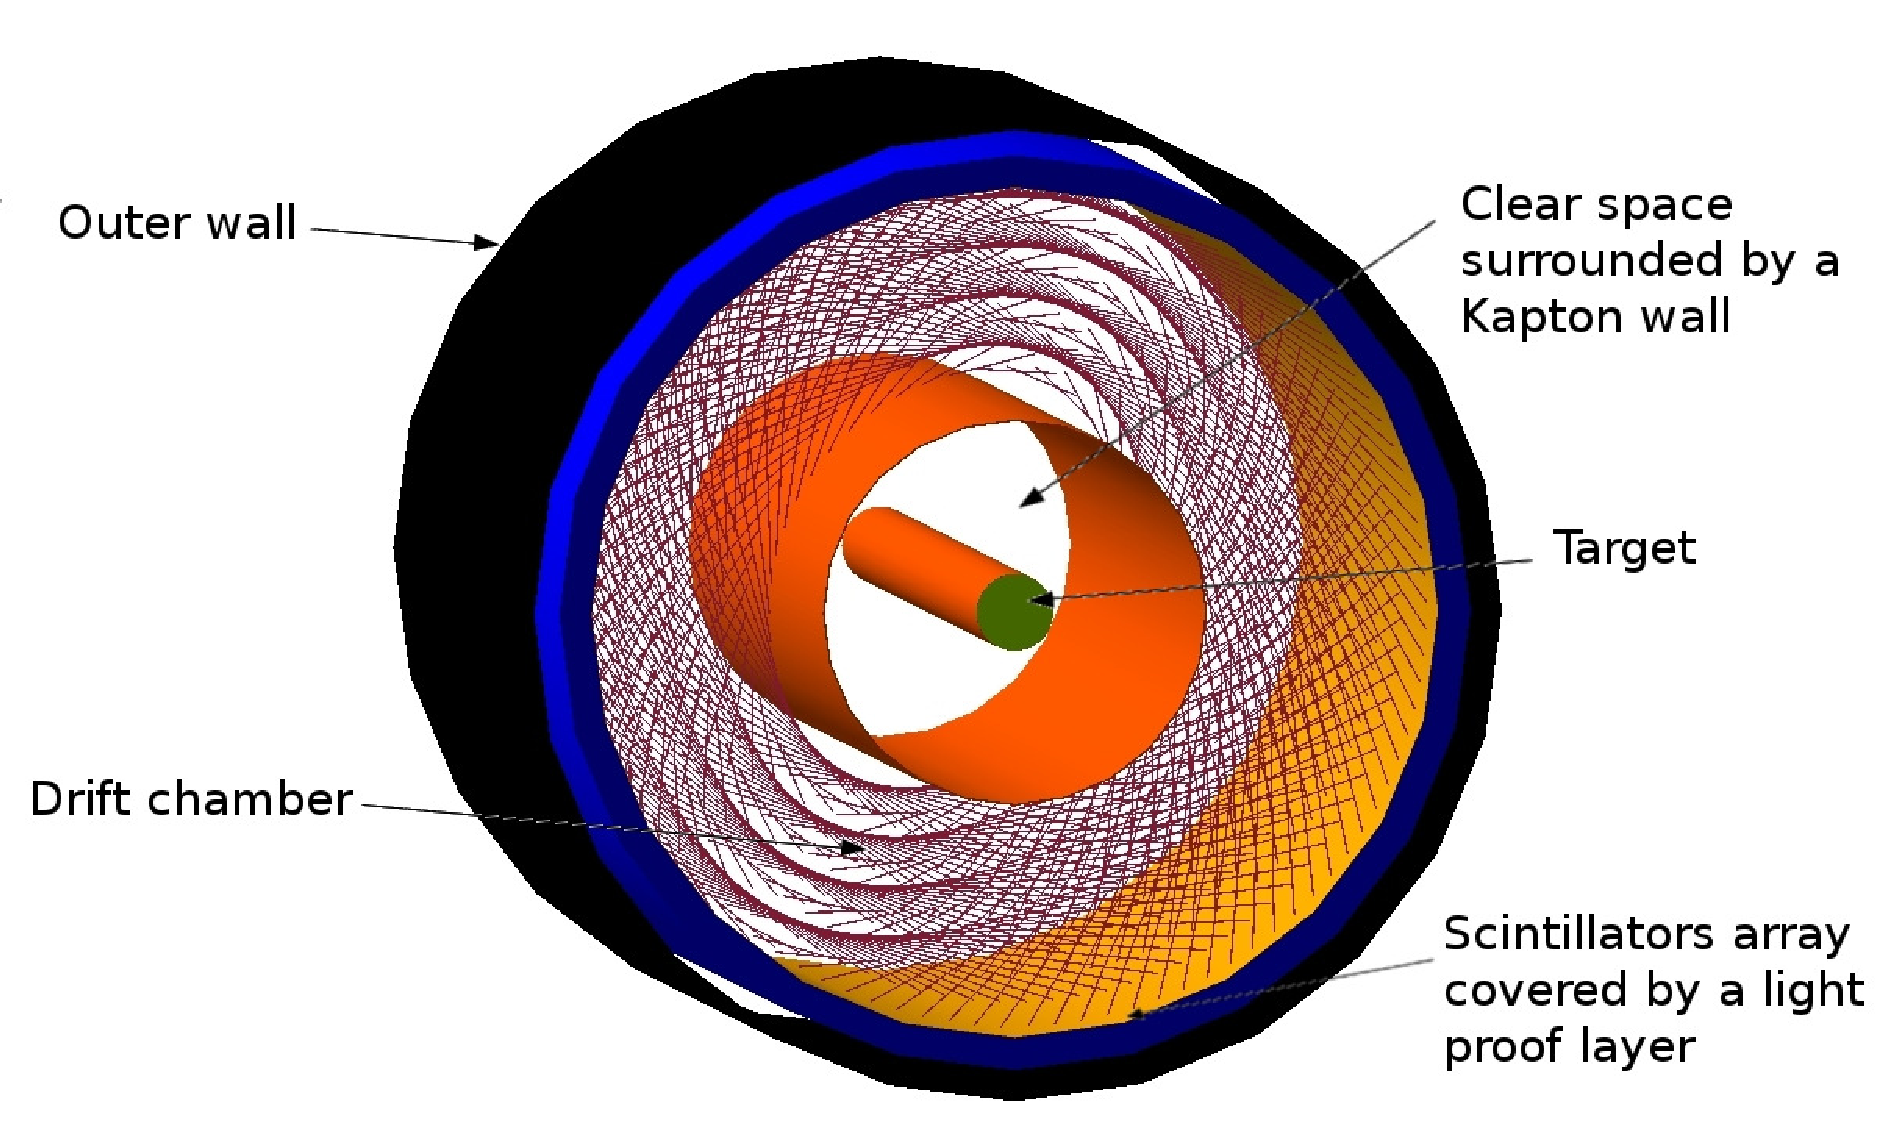
\includegraphics[angle=0, width=0.75\textwidth]{./../Detector/fig-chap2/View_det_names.pdf}
    \caption{The schematic layout of the new recoil detector design, viewed from the beam direction.}
    \label{fig:new_lay}
  \end{center}
\end{figure}

\subsection{Drift chamber}

While drift chambers are very usefull to cover large areas at a moderate price 
compared with other detectors, huge progress have been made in terms of 
rapidity to stand higher rates using better electronics, shorter distance 
between wires and optimization of the electric field over pressure ratio. Our 
design is based on other chambers developed recently. For example for the 
dimuon arm of ALICE at CERN, drift chambers with cathode planes were built in 
Orsay \cite{AliceMuonArmChamber}. The gap between sense wires is 2.1~mm and the 
distance between two cathode planes is also 2.1~mm, the wires are stretched 
over about 1~m. Belle II is building a cylindrical drift chamber very similar 
to what is needed for this experiment for which the space between wires is 
around 2.5~mm \cite{BelleIItdr}. Finally, a drift chamber with wires distant of 
1~mm is being built for the small wheel of ATLAS at CERN \cite{ATLASChamber}.  
The cylindrical drift chamber proposed for our experiment is 400~mm long, we 
therefore considered that a 2~mm gap between wires would be a rather 
conservative goal. Optimization is envisaged in the future based on experience 
with prototypes. \\

However, the radial form of the detector does not allow for 90 degrees x-y 
wires in the chamber. So we use a stereo angle between wires to determine the 
coordinate along the beam axis ($z$). It will make it possible to use a very 
thin forward end-plate to reduce multiple scattering of the outgoing 
high-energy electrons. A rough evaluation of the weight due to about 2600 
400~mm long wires is under 600~kg, which appears to be reasonable for a 
composite endplate. \\

Our drift chamber cells are composed of one sense wire made of gold plated 
tungsten surrounded by field wires, however the presence of the 5~T magnetic 
field complicates the field lines. Several structures with MAGBOLTZ 
\cite{Magboltz} are studied. Our choice now is to choose a conservative 
configuration as shown in Fig.~\ref{fig:drift_cell}. The sense wire is 
surrounded by 8 field wires placed equidistantly from it. The distance between 
the sense and field wires is constant and equal to 2~mm. Two adjacent cells 
share the three field wires placed between them. They are 8 layers of cells at 
increasing radius from the target. \\

\begin{figure}
  \begin{center}
    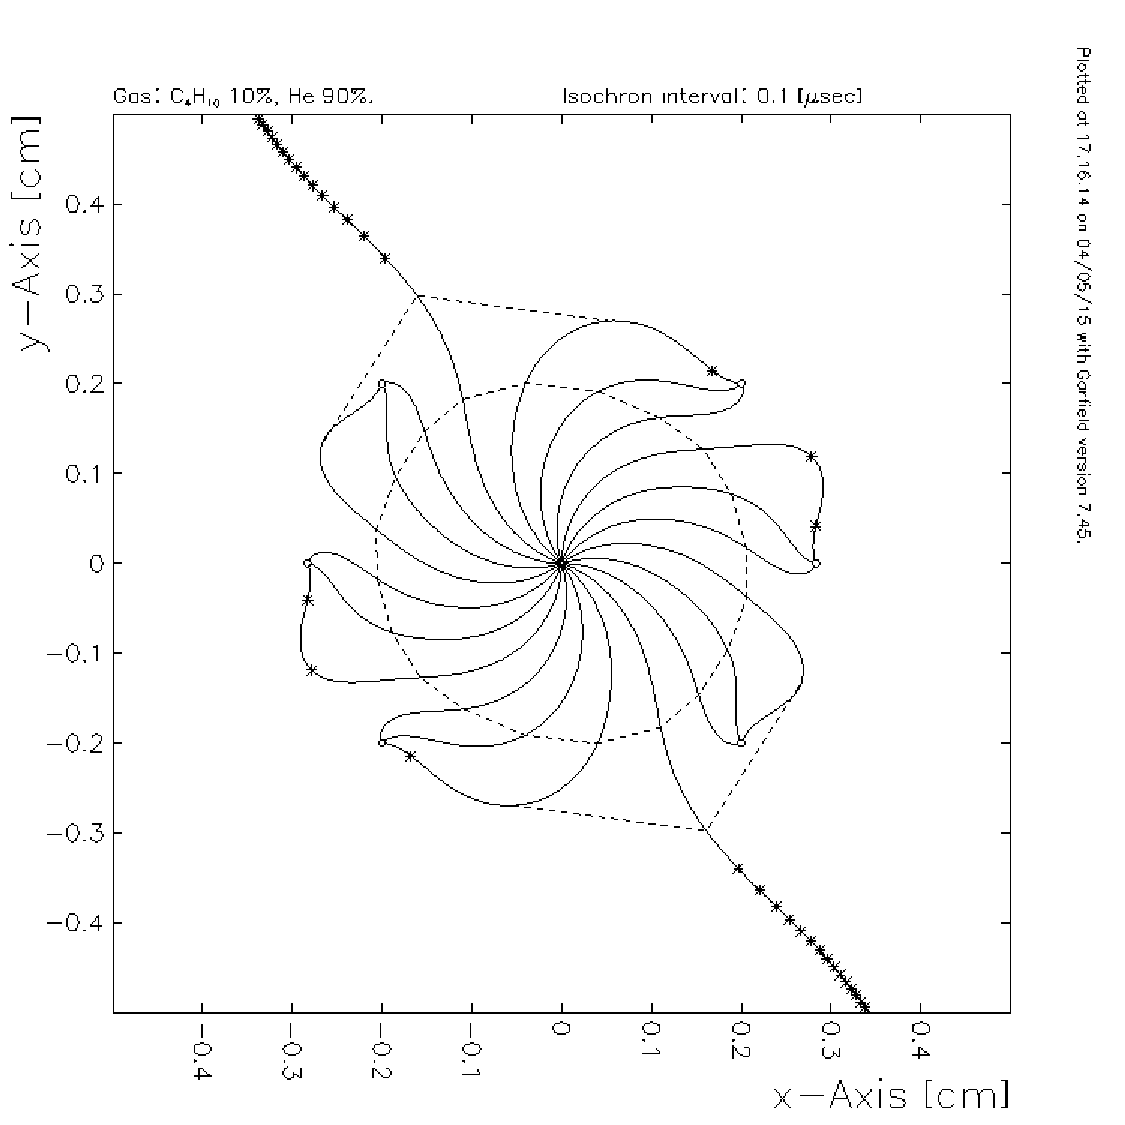
\includegraphics[angle=0, width=0.5\textwidth]{./../Detector/fig-chap2/HEISOE.pdf}
    \caption{Drift lines simulated using MAGBOLTZ \cite{Magboltz} for one sense wire (at the center) surrounded by 6 field wires. The two electric field lines leaving the cell are removed when adjusting the voltages on the wires.}
    \label{fig:drift_cell}
  \end{center}
\end{figure}

The simulation code MAGBOLTZ is calculating the drift speed and drift paths of 
the electrons (Fig.~\ref{fig:drift_cell}). With a moderate electric field, the 
drift speed is around 10~microns/ns, the maximum drift time expected is thus 
300~ns (over 3~mm). Assuming a conservative 15~ns time resolution, the spatial 
resolution will be around 200~microns. 

The maximum rates are expected for protons to be around 5~MHz for $2.10^{34}$~cm$^{-2}$s$^{-1}$, for an integration time of 300~ns and considering 8 layers of sense wires where two readout wires are about 4~mm distant, the occupancy for the inner most layer is expected around 3~\% which should be reasonable to keep a good tracking. When running with the helium 4 target, it is not necessary to detect the protons, the rate can then be highly reduced by increasing the threshold, thus making the chamber blind to protons. \\

We are currently investigating two possibilities to read out the signals from the wires.
The first possibility is to use the same preamplifier as the one developed for the CLAS inner calorimeter and improved for the Heavy Photon Search \cite{HPS} experiment installed in the Hall B. Depending on the gain in the drift chamber and the number of primary ionizations, it is possible to tune the gain of the preamplifier to adapt it to the needs of this experiment. More studies will be needed to evaluate how the gains of the chamber and the preamplifier can be tuned to ensure a noise that allows to discriminate clearly electrons from protons. The time resolution of HPS has been shown to around 1.6~ns for all crystals (Fig.~\ref{fig:HPSTreso}) which is much better than our requirements. For this task we will also use the experience from the Belle II small drift chamber electronics, that has similar requirements.

\begin{figure}
  \begin{center}
    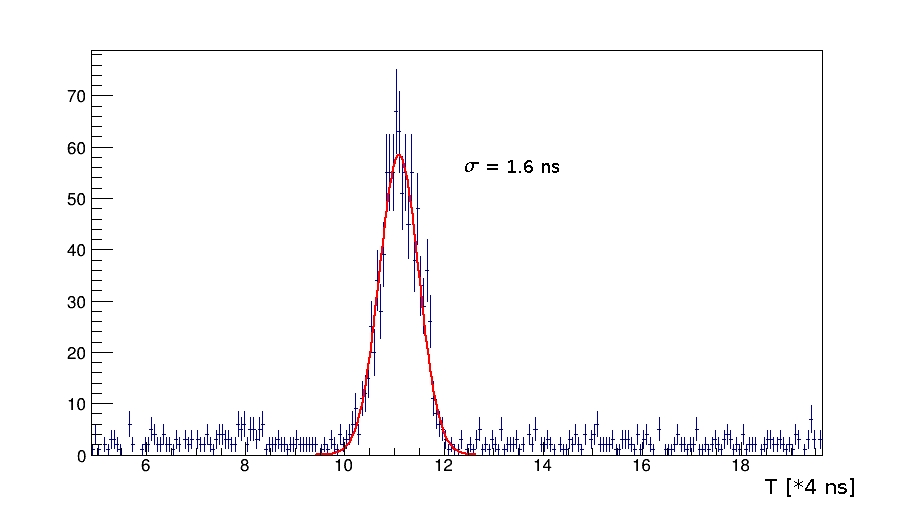
\includegraphics[angle=0, width=0.5\textwidth]{./../Detector/fig-chap2/timing_fit_gauss_3pol}
    \caption{Typical time resolution of a crystal for HPS calorimeter.}
    \label{fig:HPSTreso}
  \end{center}
\end{figure}

Another possibility would be to use the electronics used by the Micromegas of 
CLAS12, DREAM. It's dynamic range and time resolution seem to correspond to the 
need of our drift chamber. To ensure that it is the case, tests with a 
prototype will be performed.

\subsection{The scintillator array}

The scintillator array will have two main purposes. With its very good time 
resolution it will be included in the trigger to help reducing the background.  
It will also contribute to the particle identification. Its length should not 
exceed 400~mm making possible to reach a time resolution of 150~ps. It must 
also have a segmentation that will allow a good matching with the track 
reconstructed in the drift chamber. To improve our identification capabilities 
(see below) we also plan to segment the scientillators in several layers.  
Additional simulations will be done to optimize the geometry and thickness of 
the scintillators, but we show below that the simple proposed solution will 
already work for our experiment.

\section{Reconstruction scheme} \label{sec:sim}

Particle identification requires stopping the recoiling nucleus, measuring its 
time of arrival and energy deposition. The scheme used here is to measure the 
time of arrival of the particle in the scintillators along with its radius 
reconstructed by the tracking algorithm of the drift chamber. Using this method 
$\alpha$ and $^2$H have similar behavior. It is however easy to distinguish 
them using the energy deposited and the time of arrival in the scintillators.  
Moreover, if several layers of scintillators are used, the $\alpha$ will let a 
signal only in the first, making it even easier to distinguish them from the 
other particles. 


The track obtained using a helix fit is used to determine the coordinates of 
the vertex point and the transverse momentum of the particle. The energy 
deposited in the solid detector can also used to determine the kinetic energy 
of the nucleus. The feasibility and precision of the proposed vertex 
reconstruction and particle identification scheme are investigated with GEANT4 
simulation.

The simulation of the recoil detector has been implemented with the full 
geometry and material specifications. It includes a 5~Tesla homogeneous 
solenoid field. The entire detector is filled with a mixture of He(90\%) and 
iC$_4$H$_{10}$(10\%) at 1~atm which is a very light gas. It allows to reduce 
energy loss and limit the energy deposition by minimum ionizing particles.  \\

In the current study all recoil species are generated with the same 
distributions: flat in momentum from threshold up to 40~MeV ($\sim$~250~MeV/c) 
for protons and about 25~MeV for other particles; isotropic angular coverage; 
flat distribution in $z$-vertex; and a radial vertex coordinate smeared around 
the beam line center by a Gaussian distribution of sigma equal the beam 
expectation radius (0.200 mm). \\

With the requirement that the particle reaches the scintillator and with a 
40~cm length limit, there is a smoothly varying acceptance when averaged over 
the $z$-vertex position. This is shown from simulation in 
Fig.~\ref{fig:acceptance} for the lightest and heaviest recoil nuclei. However, 
this is a conservative estimate, as with tracking only information a more 
elaborate PID scheme may be able to accommodate a larger acceptance for lower 
energy recoils.\\

\begin{figure}[ht!]
    \begin{center}
        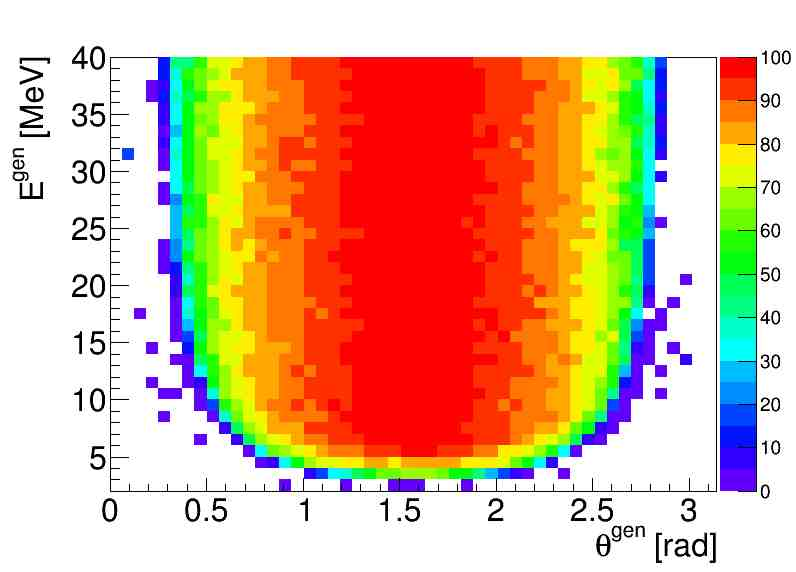
\includegraphics[width=0.45\textwidth]{./../Detector/fig-chap2/Bare_3atm_1atm_Proton_Acceptance}
        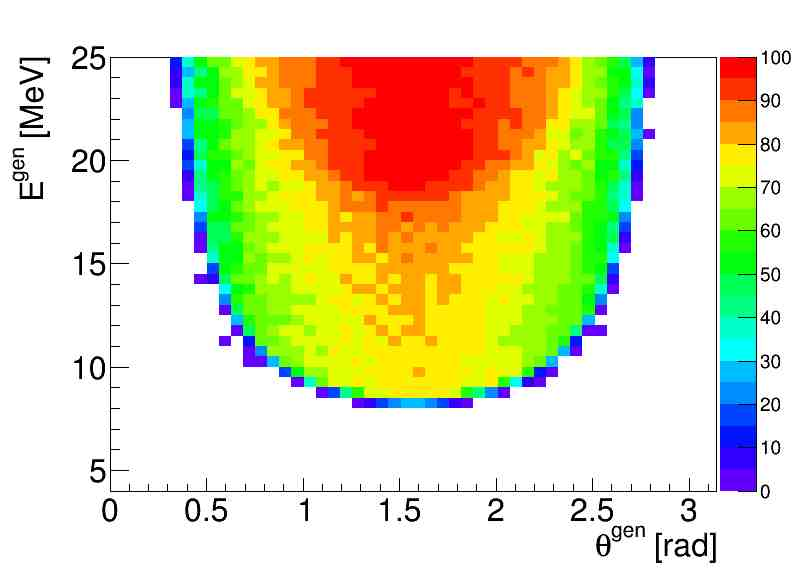
\includegraphics[width=0.45\textwidth]{./../Detector/fig-chap2/Bare_3atm_1atm_Alpha_Acceptance}
        \caption{Simulated recoil detector acceptance, for protons (left) and $^4$He (right), requiring energy deposition in the scintillators array. \label{fig:acceptance}}
    \end{center}
\end{figure}

First, the tracking capabilities of the recoil detector are investigated 
assuming a spatial resolutions of 200~$\mu$m for the drift chamber. The wires 
are strung in the $z$-direction with a stereo angle of 10$^\circ$. For 
particles stoped in the scintillators, the resulting difference between 
generated and reconstructed variables from simulation is shown in 
Fig.~\ref{fig:tracking} for $^4$He particles. The momentum for protons and 
$^4$He was also reconstructed (Fig.~\ref{fig:presolution}) from the radius of 
the helix assuming a uniform 5~T field. From these plots, it is clear that the 
resolutions required are fulfilled. \\

\begin{figure}[ht!]
    \begin{center}
        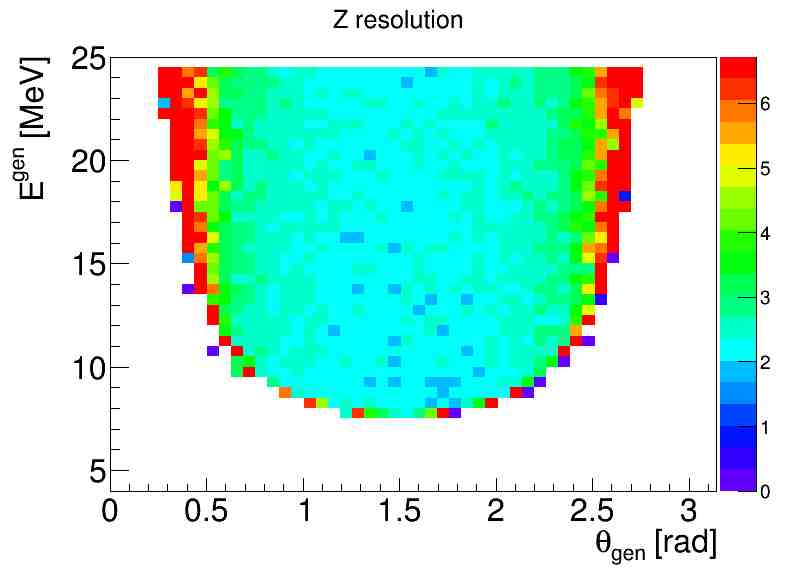
\includegraphics[height=4.5cm, width=0.32\textwidth]{./../Detector/fig-chap2/Bare_3atm_1atm_Alpha_ResoZ}
        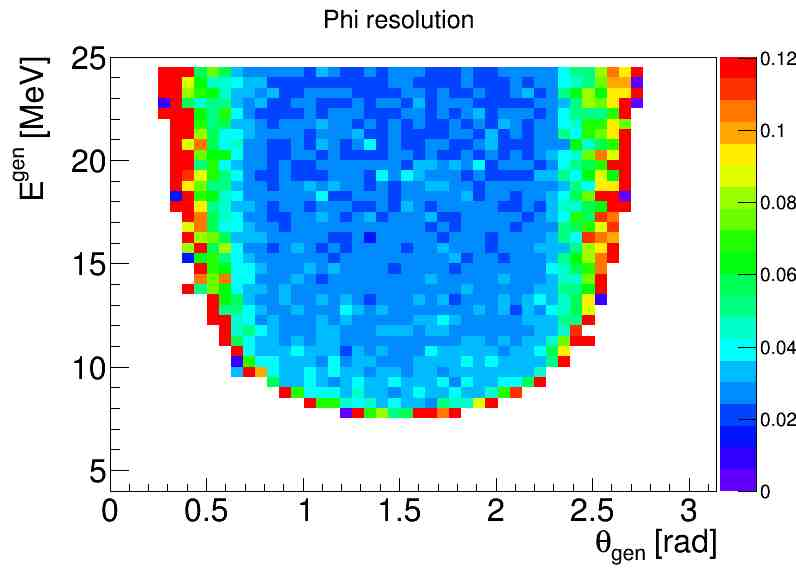
\includegraphics[height=4.5cm, width=0.32\textwidth]{./../Detector/fig-chap2/Bare_3atm_1atm_Alpha_ResoPhi}
        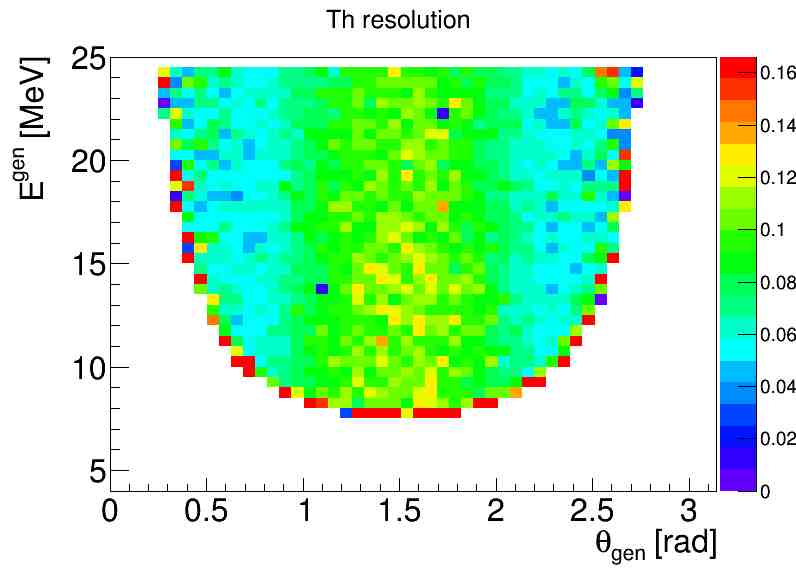
\includegraphics[height=4.5cm, width=0.32\textwidth]{./../Detector/fig-chap2/Bare_3atm_1atm_Alpha_ResoTh}
        \caption{Simulated resolutions, integrated over $z$ for $^4$He, of the $z$-vertex (in mm) and the polar and azimuthal angles (in rad) for the lowest energy regime when the recoil track reaches the scintillator. \label{fig:tracking}}
    \end{center}
\end{figure}
\begin{figure}[tbp]
    \begin{center}
        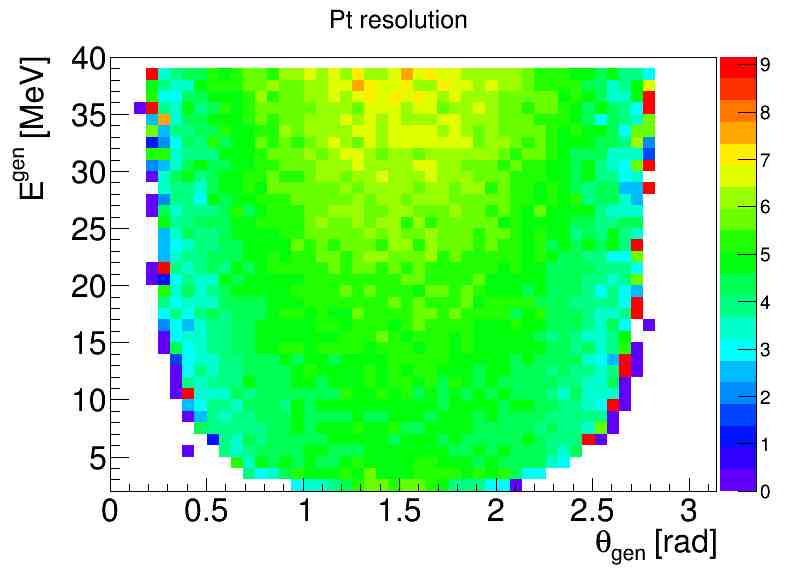
\includegraphics[width=0.45\textwidth]{./../Detector/fig-chap2/Bare_3atm_1atm_Proton_ResoPt}%proton__pdp_sigma__regime1_small.png}
        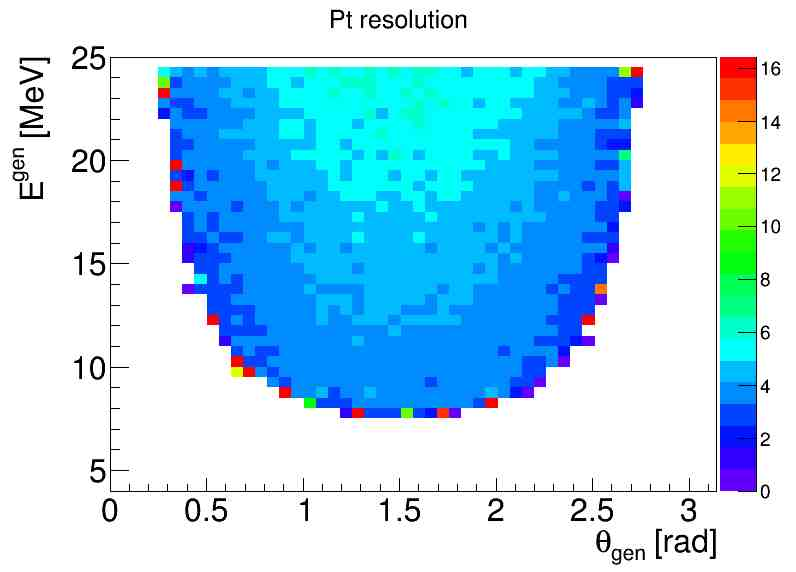
\includegraphics[width=0.45\textwidth]{./../Detector/fig-chap2/Bare_3atm_1atm_Alpha_ResoPt}%alpha__pdp_sigma__regime1_small.png}
        \caption{Simulated momentum resolutions for proton (left) and $^4$He (right) integrated over $z$, when the recoil track reaches the scintillators array.\label{fig:presolution}}
    \end{center}
\end{figure}

Next, the particle identification scheme is investigated. Assuming a 150~ps 
resolution of the scintillator and an energy resolution of 10\%, clean 
separation of three of the five nuclei is shown in Fig.~\ref{fig:SIMtof} which 
represents the time of arrival in the scintillator as a function of the 
reconstructed radius in the drift chamber. While not directly a concern for our 
experiment, we note that using energy deposition versus the radius 
reconstructed in the drift chamber one can separate $^2$H from $\alpha$. Also, 
the comparison of the energy deposited versus the radius and the angle $\theta$ 
can be used to improve the results.\\

\begin{figure}[ht!]
    \begin{center}
        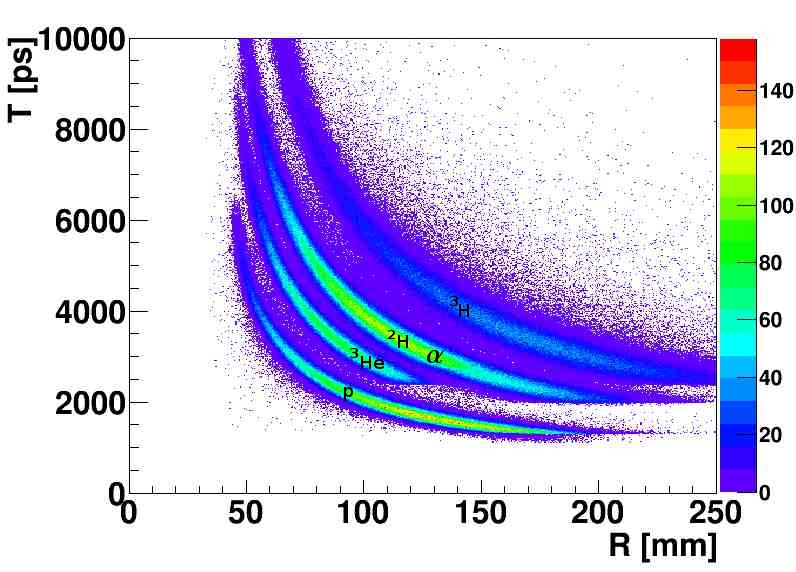
\includegraphics[width=0.7\textwidth]{./../Detector/fig-chap2/Bare_3atm_1atm_RvsTime_named}
        \caption{Simulated time of flight at the scintillator versus the reconstructed radius in the drift chamber. The bottom band correspond to proton, next band is the $^3$He nuclei, $^2$H and $\alpha$ are overlapping in the third band, the uppermost band is $^3$H.\label{fig:SIMtof}}
    \end{center}
\end{figure}


We finally found particle identification efficiency of 99\% for protons, 95\% 
for $^3$He and 98\% for $^3$H. This conservative analysis suggests that the 
proposed reconstruction and particle identification schemes for this design are 
quite promising. Studies, using both software and prototyping, are ongoing to 
determine the optimal detector parameters to minimize the detection threshold 
while maximizing particle identification efficiency. The resolutions presented 
above have been implemented in a fast Monte Carlo used in the next section to 
evaluate our discovery potential.

\section{Drift chamber prototype}


